% Autogenerated translation of README.md by Texpad
% To stop this file being overwritten during the typeset process, please move or remove this header

\documentclass[12pt]{book}
\usepackage{graphicx}
\usepackage{fontspec}
\usepackage[utf8]{inputenc}
\usepackage[a4paper,left=.5in,right=.5in,top=.3in,bottom=0.3in]{geometry}
\setlength\parindent{0pt}
\setlength{\parskip}{\baselineskip}
\setmainfont{Helvetica Neue}
\usepackage{hyperref}
\pagestyle{plain}
\begin{document}

\chapter*{Mixed Kinematics and Camera Based Vehicle Dynamic Sideslip Estimation for an RC Scaled Model}

\emph{This paper, written by Conno Kuyt and Matteo Corno, has been published and presentaed at the 2018 IEEE Conference on Control Technology and Applications (CCTA) Copenhagen, Denmark, August 21-24, 2018.}

https://ieeexplore.ieee.org/abstract/document/8511487

\section*{Abstract}

Vehicle side slip angle is at the basis of many vehicle dynamics control systems. Many methods are available to estimate side-slip angle using on board sensors (usually accelerometers and gyros). The technical advances pertaining autonomous vehicles made an additional kind of sensor available: cameras. This study develops a mixed kinematic vision-based side slip angle estimation. The proposed algorithm merges the information of a commercial grade inertial measurement system, wheel encoders and information from a camera. The camera measurement are integrated in a Kalman filter observer. The paper implements and tests the approach on an instrumented RC scale vehicle, comparing the proposed approach against a kinematic based estimation. Experimental results show a decrease of a factor between 2 and 10 (depending on the type of maneuver) of the estimation mean squared error.

\section*{Introduction}

To improve traffic and vehicle safety and reduce related casualties, control systems are constantly being developed to assist drivers. These developments have been moving towards full vehicle control automation.  One of the challenges is to maximize the operational regime of the control systems to be on the edge or even outside of the stable envelope of the tires to be able to avoid accidents in extreme emergency situations. As a vehicle moves outside of the stable envelope the tires lose grip and start slipping, known as \emph{drift motion}. Analyses of drift motion led to a better understanding of both the dynamics as well as its potential practical use in vehicle dynamic control design. Studies on race driver behavior inspired novel design approaches for automated drift controllers. The control objectives of the studies on automated drift control included the stabilisation of the vehicle at a reference sideslip angle. The experimental setups in these studies used a state estimator that relies on external and costly on-board sensors such as differential GPS. This approach to estimation is not feasible in an automotive industry standard production setting. 

Sideslip estimation based on \emph{stock} sensors (low-cost industry standard sensors) is a widely investigated topic. Examples of these sensors are wheel angular velocity encoders, steering angle encoders, IMU's and (low-cost) GPS receivers. There are mainly two general approaches to side slip angle estimation: black-box and physical-based approaches. The black-box approach is based on data driven models, such as neural networks. Physical-based  approaches are instead based of first principle models. These can be further classified in kinematic and dynamic models. Kinematic approaches rely on a simple vehicle model description that correlates basic kinematic quantities. These models are independent from specific parameters (such as tyre parameters) but suffer from a lack of observability for small yaw rates. Dynamic approaches include knowledge of the vehicle  and tyre parameters. They solve the issue of observability at the cost of a greater modelization effort. 

Most of the approaches in the literature employ standard inertial or mechanical sensors (encoders). Recently, thanks to the introduction of advanced driver assistance systems (ADAS) cameras have become standard sensors in cars. Currently, cameras are mainly used to detect other road users and obstacles in sufficient detail to make tactical decisions. However, the data coming from the cameras can  be used to extract motion information to support sideslip estimation.

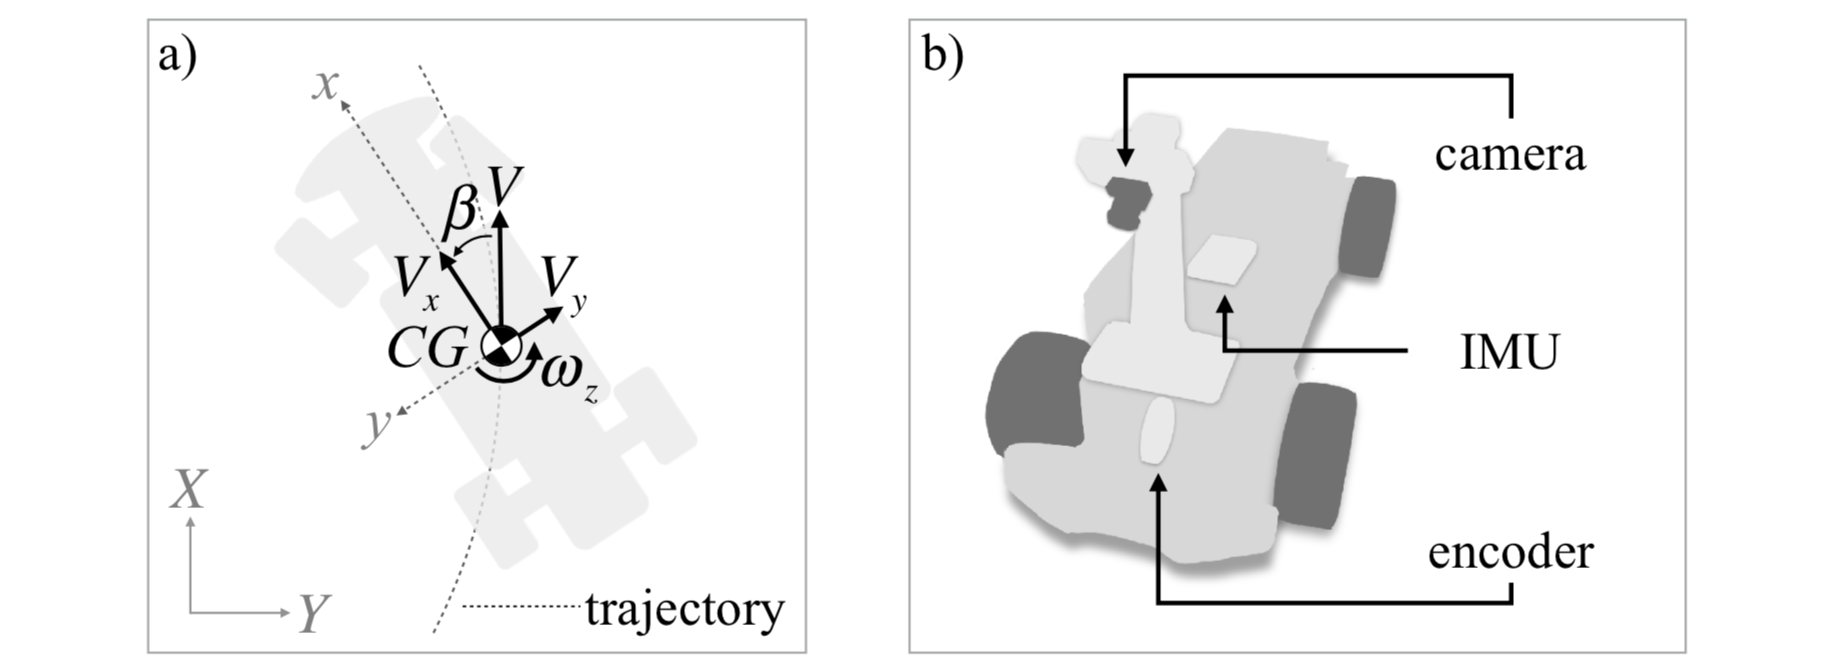
\includegraphics{objectives.png}

This paper proposes a side slip estimation algorithm that fuses the information from classical sensors with the information provided by a camera. Starting from the approach of \\\href{https://www.sciencedirect.com/science/article/abs/pii/S0967066117301491}{Selmanaj et al. 2017}, the proposed Kalman filter fuses the information processed by a computer vision algorithm with a kinematic based side slip angle estimation. The algorithm is developed for an RC model car  (see the above figure) equipped with an 3 DoF Inertial Measurement Unit, wheel axle encoders, and a mono-camera. 

Other authors have investigated the same problem. In particular, \href{http://proceedings.asmedigitalcollection.asme.org/proceeding.aspx?articleid=2591696}{Botha et al. 2016} develops a method based on a stereo camera; \href{http://proceedings.asmedigitalcollection.asme.org/proceeding.aspx?articleid=1648272}{Harchut et al. 2009} employs a mono-camera and, similarly to our contribution, uses colored objects placed on the road to estimate sideslip angle. However the cited approach only uses the information from the camera and no sensor fusion is carried out. Finally, \href{https://ieeexplore.ieee.org/document/6548052}{Wang et al. 2012} run a fusion algorithm that however requires information on the vehicle dynamic model (namely cornering stiffness). Differently from the previous contributions on the subject matter, the approach employed in this paper uses a mono camera and runs a kinematic-based sensor fusion. 

The paper is structured as follows: Section 1 discusses the basic rationale of the algorithm. Section 2 details the algorithm implementation. The focus of this contribution is on the sensor fusion approach, and not the computer vision algorithm for which a standard approach in the literature is employed.  Section 3 describes the experimental setup that is then employed in Section 4 for the final validation. 

\end{document}
